

\documentclass[12pt]{report}
\usepackage[a4paper,width=150mm,top=25mm,bottom=25mm,bindingoffset=6mm, includefoot, includehead]{geometry}
\usepackage[backend=bibtex]{biblatex} %Imports biblatex package
\addbibresource{bibfile.bib} %Import the bibliography file


\usepackage[utf8]{inputenc}
\usepackage[italian]{babel}
\usepackage{alphabeta}
\usepackage{minted}
\usepackage{graphicx}
\graphicspath{ {./resources/} }

\usepackage{array} % per tabelle


\usepackage{amsfonts}
\usepackage{amsmath}
\usepackage{amssymb,amsmath,color}
\usepackage{graphicx}
\usepackage{float}
\usepackage{standalone}
\usepackage{changepage}
\usepackage{longtable}
\usepackage{colortbl}
\usepackage{graphicx}
\usepackage{fancyhdr}
\usepackage{float}
\usepackage{color}
\usepackage[nottoc]{tocbibind}
\usepackage{xcolor}
\usepackage{titlesec}
\usepackage{amssymb}

\usepackage{pdfpages}

\usepackage{placeins} %for floatBarrier

\addtolength{\skip\footins}{2pc plus 5pt}

\usepackage{hyperref}

\hypersetup{
    citecolor=black,
    colorlinks=true,
    linkcolor=black,
    filecolor=magenta,      
    urlcolor=black,
    pdftitle={Ottimizzazione Applicazioni Angular},
    pdfpagemode=FullScreen,
    }
    
\usepackage{minted}
\usemintedstyle{manni}

\newcommand\myemptypage{
    \null
    \thispagestyle{empty}
    \newpage
}


\usepackage{pgfplots}


\usepackage{fancyhdr}
% Stile di pagina
\pagestyle{fancy}
\definecolor{LightGray}{gray}{0.9}
\usemintedstyle{colorful}

\fancyhf{}
\fancyhead[LE]{\nouppercase{\rightmark\hfill\leftmark}}
\fancyhead[RO]{\nouppercase{\leftmark\hfill}}%\rightmark}}
\fancyfoot[LE,RO]{\hfill\thepage\hfill}


% Stile dei titoli dei capitoli
\definecolor{gray75}{gray}{0.75}
\newcommand{\hsp}{\hspace{20pt}}
\titleformat{\chapter}[hang]
{\Huge\bfseries}
{\thechapter\hsp\textcolor{gray75}{}\hsp}
{0pt}
{\Huge\bfseries}


\renewcommand{\contentsname}{Indice}


\begin{document}
\begin{titlepage}
\begin{center}
{{\Large{\textsc{Alma Mater Studiorum $\cdot$ Universit\`a di
Bologna}}}} \rule[0.1cm]{15.8cm}{0.1mm}
\rule[0.5cm]{15.8cm}{0.6mm}
{\small{\bf SCUOLA DI INGEGNERIA E ARCHITETTURA\\
Corso di Laurea in Ingegneria Informatica }}
\end{center}
\vspace{15mm}
\begin{center}
{\LARGE{\bf Applicazioni Web per Smart Home }}\\
\vspace{3.8mm}
{\LARGE{\bf basate su Tecnologia Angular}}\\
\vspace{3mm}
\end{center}
\vspace{40mm}
\par
\noindent
\begin{minipage}[t]{0.47\textwidth}
{\large{\bf Relatore:\\
Chiar.mo Prof.\\
Paolo Bellavista}}
\vspace{1cm}
\end{minipage}
\hfill
\begin{minipage}[t]{0.47\textwidth}\raggedleft
{\large{\bf Presentata da:\\
Matteo Longhi}}
\end{minipage}
\vspace{20mm}
\begin{center}
{\large{\bf Sessione 3\\
Anno Accademico 2021-2022}}
\end{center}
\end{titlepage}




\newpage
\thispagestyle{empty}
\newpage


\newcommand\blankpage{%
    \null
    \thispagestyle{empty}%
    \addtocounter{page}{-1}%
    \newpage}
\blankpage{}



\tableofcontents 


%%%%%%%%%%% Abstract %%%%%%%%%%%%
\newpage
\thispagestyle{empty}
\mbox{}
\newpage

\begin{abstract}

    Angular è una delle principali tecnologie utilizzate in ambito enterprise per la realizzazione di web Application ad alta manutenibilità e performance.In questo documento verranno disquisite le funzionalità legate alla ottimizzazione delle performance offerte dalla libreria, la gestione e aggiornamento del DOM e le possibili strategie adottabili per la sua ottimizzazione 
\end{abstract}
%%%%%%% INTRODUCITON %%%%%%%%%%%%%%%% 
\addcontentsline{toc}{chapter}{Introduzione}
\chapter*{Introduzione}
In questo elaborato verranno discusse le metodologie con cui ottimizzare le prestazioni del front end di applicazioni web.
In particolare, verranno discusse le motivazioni per cui è importante farlo. Verrà discusso lo stato attuale delle applicazioni nel web con particolare riguardo per l'ottimizzazione dei tempi di caricamento delle pagine.
\newline
L'obbiettivo del' elaborato è offrire un punto di vista, sullo sviluppo delle applicazioni web, che sia più inclusivo delle questioni e problematiche riguardanti le performance che, nello sviluppo web moderno, non è molto presente e viene spesso e erroneamente messo in secondo piano, quando in realtà influenza la user experience in maniera rilevante e può determinare da solo l'abbandono dell'applicativo da parte dell'utente.
\newline
Fra i tanti framework per lo sviluppo web verrà mostrato Angular. È stato scelto questo framework per la sua capacità di personalizzazione del comportamento a runtime tramite la change detection e il ciclo di vita dei componenti e, come verrà mostrato, per la sua natura rivolta alle performance.
\newline
Angular, inoltre offre allo sviluppatore un insieme di concetti completo e di alto livello, adatto allo sviluppo sia di applicazioni frontend di facciata come possono essere siti prevalentemente statici, sia a single page application data intensive che necessitano di alte performance. Inoltre angular offre un comodo ambiente di sviluppo, fornito di tool di corredo per la generazione del codice e per il tesing runtime dei suoi componenti.
\newline
Verranno analizzati i principali concetti che il framework mette a disposizione agli sviluppatori fra cui la programmazione delle interfacce orientata ai componenti,il data binding a due vie, la loro gestione a runtime, la capacità organizzativa offerta dalla libreria tramite i moduli e le modalità di implementazione della dependency injection tramite il concetto dei service.
\newline
Verrà posta particolare attenzione sul meccanismo di aggiornamento del DOM che la libreria propone,chiamato change detection.
La change detection è il meccanismo che il framework utilizza per il monitoraggio e aggiornamento della view.
Verrà mostrato il suo funzionamento, le modalità con cui la libreria lo implementa, le possibilità di ottimizzazione tramite la strategia onPush e le accortezze da prendere in fase di sviluppo per un corretto utilizzo dello stesso.
\newline
A fini dimostrativi, verrà incluso il progetto di un applicazione per la gestione elettronica delle ricette di cucina che metta in mostra le capacità del framework, con particolare riguardo verso il meccanismo di change detection. Verranno mostrati i requisiti, la struttura dell'applicazione e la sua progettazione con test conclusivi delle prestazioni.
L'applicazione ha come obbiettivo quello di soppiantare il classico libro di ricette tenuto in casa realizzandone una versione elettronica, offrendo inoltre la possibilità di creare gruppi famiglia all'interno del quale condividere le ricette




%%%%%%%%%% Chapters %%%%%%%%%%
%%%%%%% WHY ANGULAR %%%%%%%%%%%%%%%% 
\chapter{Il web ad oggi}
\section{Perché ottimizzare la propria interfaccia web?}
Le tecnologie per la produzione di applicazioni web si sono evolute esponenzialmente da quando il web era ancora un progetto pensato per scambiare documentazione scientifica in modalità elettronica. Oggi il web viene utilizzato per gli scopi più disparati, dal promuovere il proprio business a offrire veri e propri servizi ad alto traffico e scalabilità.
Molte compagnie basano il proprio business esclusivamente sul mondo web, si pensi ad un sito ecommerce o a piattaforme di condivisione come i social, Chi invece gestisce business esterni sfrutta il web e le piattaforme sviluppate su di esso per promuovere la propria attività, in un contesto diventato ormai essenziale per ogni tipo di business.
\newline
Pensiamoci, qual'è  la prima cosa che facciamo quando necessitiamo di informazioni su un particolare prodotto o servizio? oppure abbiamo bisogno di riempire un vuoto informativo in maniera tempestiva?  interroghiamo l'oracolo del nuovo millennio Google in cerca di risposte.
\newline
Il mondo web si è espanso cosi tanto da diventare un qualcosa di normale e scontato nella nostra vita quotidiana e con tante realtà che ormai spostano le loro vetrine e i loro contenuti informativi su questa tecnologia, e offrono user experience sempre più avanzate, gli utenti sono diventati sempre più esigenti in termini di performance e tempi di risposta da parte di questi servizi.Secondo uno studio condotto nel 2018 da Google, la probabilita che un utente abbandoni il sito aumenta in maniera esponenziale in base al tempo di caricamento delle pagine.\cite{mobile-page-speed}
\newline
\begin{figure}[H]
\centering
   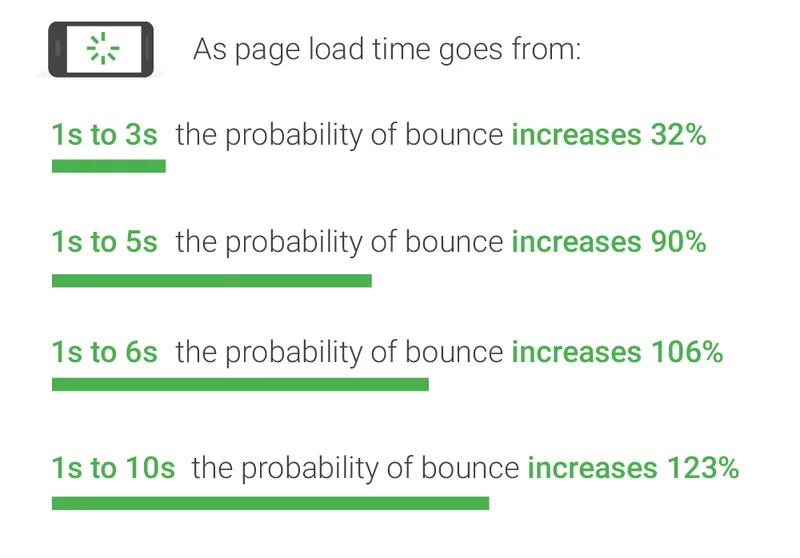
\includegraphics[scale=0.5]{resources/mobile-page-speed-new-industry.png}
\cite{mobile-page-speed}
\caption{probabilità di abbandono del sito in relazione al tempo di caricamento}
\end{figure}
Inoltre, più della metà delle richieste effettuate a questi servizi avviene da device mobile e per il 70\% dei siti analizzati i tempi di caricamento ammontano a più di 5 secondi. \cite{mobile-page-speed}


\section{Il web in numeri: statistiche}
Se si da uno sguardo alle statistiche ci si può accorgere che la maggior parte dei siti non dedica le giuste attenzioni all'ottimizzazione del proprio servizio, in particolare secondo uno studio effettuato da tooltester.com:
\begin{itemize}
    \item Il tempo di caricamento medio delle pagine è di 2.5 secondi per i device desktop e 8 per i device mobile.
    \item Il delay del primo contatto con l'utente è di 12.73 millisecondi per i device desktop e di 59.73 per i device mobile
    \item Le pagine  impiegano un tempo medio di caricamento superiore del 70.9\% su device mobile rispetto che su device desktop
    \item Gli utenti di device mobile sono al primo posto nella classifica di abbandono delle pagine con una percentuale di 56.8\% 
    \item il settore delle scienze possiede il rateo di abbandono più alto con una percentuale di 66.37\%
    \item Di tutte le tipologie di device (desktop/tablet/mobile) il tablet è quello con il minor numero di sessioni all'anno con una percentuale di 2.3%
\end{itemize}
\begin{figure}[H]
   \centering
   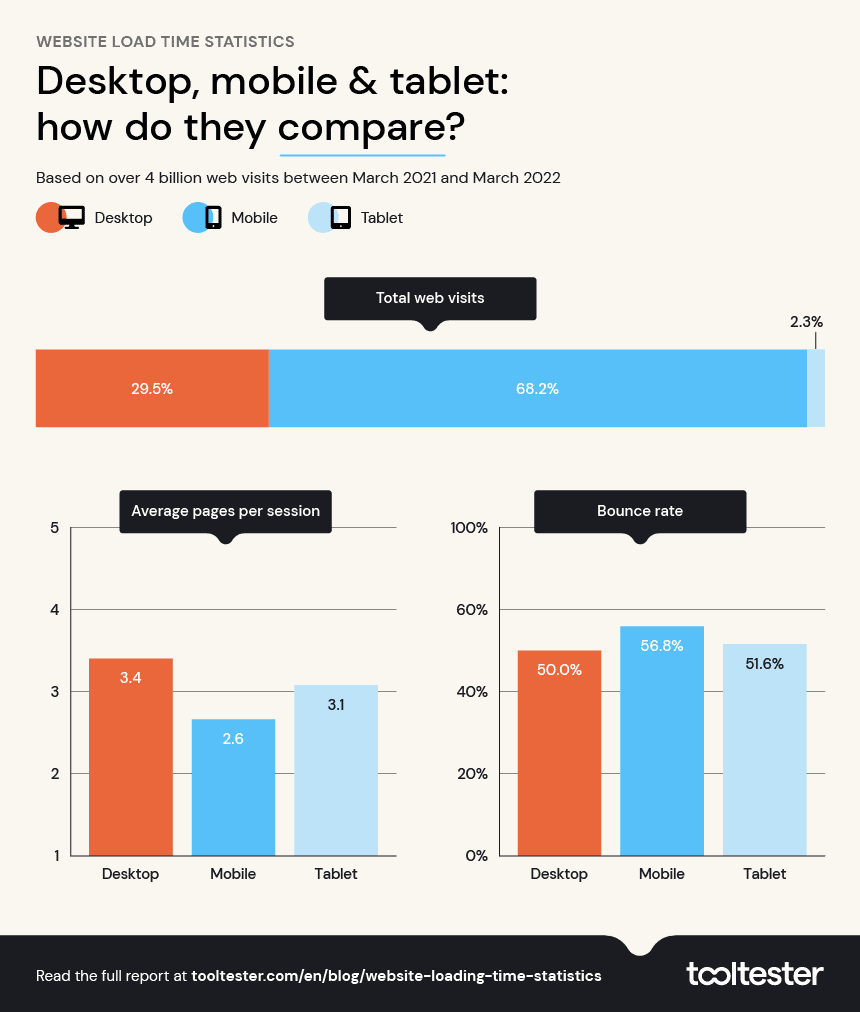
\includegraphics[scale=0.25]{resources/website-load-time-statistics-desktop-mobile-tablet.png}
\cite{website-loading-time-statistics}
\caption{Statistiche di visualizzazione pagine web}
\end{figure}


   
\section{Perché Angular?}
Date queste premesse l'elaborato si pone come obbiettivo quello di mostrare le funzionalità di ottimizzazione delle performance che il framework angular offre agli sviluppatori.
\newline
Nato nel 2016 come evoluzione di angularjs e mantenuta da un team indipendente di sviluppatori google, la libreria viene ormai adottata sia per lo sviluppo di single page application ad alte prestazioni sia per la costruzione di frontend web.
\newline
La libreria offre molte possibilità agli sviluppatori
\begin{itemize}
    \item La possibilita di fare testing realtime dell'applicazione
    \item Alte prestazioni offerte dal meccanismo di change detection
    \item Alta flessibilità e scalabilità delle applicazioni
\end{itemize}
La libreria viene inoltre utilizzata da molte grandi realtà quali IBM Samsung e Paypal
\newline
\begin{figure}[H]
   \centering
   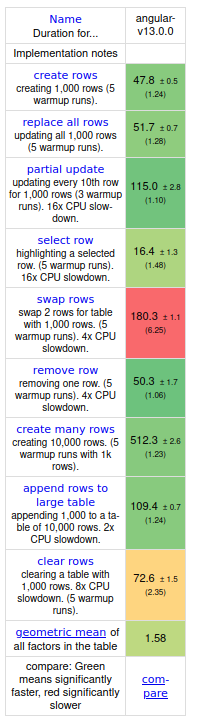
\includegraphics[scale=0.4]{resources/angular-performance.png}
\caption{test prestazioni libreria angular}
\end{figure}

%%%%%%% ANGULAR OVERVIEW %%%%%%%%%%%%%%%% 
%%%%%%INTRODUZIONE
\chapter{Angular, libreria e funzionalità}
\section{Introduzione alla tecnologia}
Angular è una libreria per lo sviluppo di interfacce web di tipologia s.p.a. (single page application) con paradigma a componenti strutturata per lo sviluppo di software ad alta manutenibilità e prestazioni.

Offre diverse funzionalità tra cui:
\begin{itemize}
    \item Sviluppo a componenti concepiti come singoli elementi di visualizzazione dei dati 
    \item Dependency injection 
    \item Possibilità di strutturazione dei componenti in raggruppamenti chiamati moduli
    \item Gestione degli eventi e possibilità di generazione degli stessi
    \item Routing tra i componenti che compongono la web-app
    \item Rendering dei componenti del DOM a runtime con monitoraggio delle variazioni e conseguente aggiornamento tramite change detection
\end{itemize} 
Le applicazioni Angular sono composte da un insieme di componenti organizzati in moduli che vengono renderizzati in una struttura ad albero, i componenti possono condividere dati tramite le properties e gli eventi.
\newline
\newline
La dependency injection è realizzata tramite i service, classi typescript istanziate dal framework il cui scopo è fornire ai componenti la logica applicativa complessa necessaria al loro funzionamento.
\newline
\newline
I componenti e i service sono raggruppati in moduli i quali fungono da elemento organizzativo dell'applicazione, i moduli stessi possono importare ed esportare componenti e servizi.
\newline
\newline
Il framework consente di effettuare il routing fra i vari componenti dell'applicazione che vengono renderizzati all'interno del DOM, in questo modo è possibile far variare i componenti visualizzati a schermo in base all iterazione con l'utente.
\newline
\newline
Tramite il meccanismo di Change detection, la libreria Angular è in grado di rilevare le modifiche effettuate alle proprietà dei componenti e aggiornare il DOM di conseguenza.
\newline
\newline
La libreria è distribuita come modulo Node.js e sfrutta npm (node packet manager) per la gestione delle dipendenze e l'istallazione di librerie di componenti angular aggiuntivi come per esempio la libreria di componenti nebular.
\newline
\newpage
%%% COMPONENTI STRUTTURA
\section{Componenti Angular}
I componenti rappresentano l'elemento base di un'applicazione Angular e sono composti da 3 elementi principali:
\begin{itemize}
    \item Una classe Typescript che ne implementa il comportamento e le proprietà 
    \item Un template HTML che ne definisce la vista renderizzata all'interno del DOM 
    \item Un file css che ne definisce lo stile
\end{itemize}
Il comportamento dei componenti viene fornito da una direttiva Component che fornisce i metadati necessari alla creazione gestione e eliminazione del componente tra cui:
\begin{itemize}
    \item Il CSS selector
    \item Il template del componente
    \item Il foglio di stile 
    \item I provider degli eventuali servizi di cui il componente potrà usufruire
\end{itemize}
In particolare è proprio il @Component decorator che identifica la classe Typescript come componente alla libreria angular, il quale senza non viene riconosciuto come tale.
\newline
Una parte fondamentale di ogni componente è il CSS selector che è il nome con cui viene riconosciuto dalla libreria e indica di renderizzare il componente ogni qualvolta viene trovato il corrispettivo tag.
\newline
\subsection{Angular template}
Il template definisce ciò che viene renderizzato nel DOM all'istanziazione,
al suo interno è possibile sfruttare il data binding dei componenti  per referenziare le proprietà definite nella classe typescript e sfruttare le direttive Angular per rendere dinamica la costruzione del DOM. 
\newline
\newline
\begin{figure}[H]
    \centering
    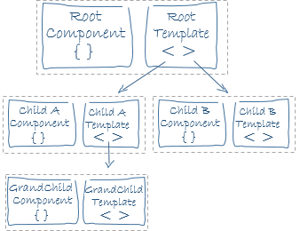
\includegraphics[scale=1]{resources/component-tree.png}
    \cite{angular-doc}
    \caption{struttura albero dei componenti}
\end{figure}

Il template di un componente e la sua classe typescript formano una view, la quale può includere altre view al suo interno in una struttura gerarchica ad albero.
\newline
Il template di un componente angular è scritto in codice HTML esteso dalla sintassi Angular per il template, la quale si occupa di alterare il DOM a seconda della logica applicativa e della variazione dei dati.
Come già anticipato, all'interno del template è possibile sfruttare:
\begin{itemize}
    \item Direttive per applicare logica al rendering del component (ngFor)
    \item Pipe per trasformare i dati prima di mostrarli a schermo 
    \item Data binding tra proprietà della classe e template
\end{itemize}
Le direttive sono classi typescript contenenti il decorator @directive che consentono di rendere il template dei componenti dinamico e si suddividono in due tipologie:
\begin{itemize}
    \item Direttive strutturali
    \item Direttive attributo
\end{itemize}
Le direttive strutturali alterano il DOM aggiungendo rimuovendo o modificando elementi come le direttive ngFor e ngIf,
mentre le direttive attributo alterano il DOM modificando il valore di singoli attributi.
\newline
\newline
Le pipe sono strumenti attraverso i quali è possibile manipolare i dati da mostrare nel DOM tramite particolari sequenze di istruzioni come per esempio la formattazione di dati nel formato locale dell'utente oppure la formattazione di valute.
\newline
\newline
Una delle operazioni più tediose e inclini alla generazione di errori nelle interfacce web è la necessità di collegare i dati mostrati all'interno dell'interfaccia con ciò che viene manipolato dalla logica applicativa. Tramite il data binding la libreria Angular automatizza questo processo come mostrato nell'immagine sottostante
\newline
\newline
\begin{figure}[H]
    \centering
    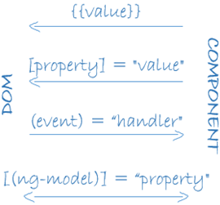
\includegraphics[scale=1]{resources/databinding.png}
    \cite{angular-doc}
    \caption{Modalità di funzionamento data binding}
\end{figure}
nell'immagine viene mostrata la possibilità di implementazione del data binding in 3 possibili modalità:
\begin{itemize}
    \item Monodirezionale dal component al dom
    \item Monodirezionale dal dom al component
    \item Bidirezionale
\end{itemize}
In questo modo viene automatizzata una procedura molto onerosa e che molto spesso rende illeggibili le interfacce di molte applicazioni web
%%%%%%% CICLO DI VITA COMPONENTI
\section{Ciclo di vita dei componenti}
I componenti Angular seguono il seguente lifecicle:

\begin{itemize}
    \item Istanziazione del componente e renderizzazione dello stesso e dei componenti figli all'interno del DOM
    \item Aggiornamento del componente secondo la strategia di aggiornamento al cambio delle proprietà dello stesso
    \item Distruzione del componente e dei rispettivi componenti e conseguente rimozione del componente dal DOM
\end{itemize}

È possibile definire comportamento aggiuntivo del componente ad ognuna delle fasi del ciclo di vita implementando i rispettivi metodi definiti dalla direttiva Component.
I metodi sono i seguenti:

\begin{itemize}
    \item ngOnInit() si occupa del rendering nel DOM del componente, chiamato una volta sola alla renderizzazione  del componente
    \item ngOnChanges() si occupa di aggiornare il componente quando la libreria modifica almeno una delle proprietà del componente
    \item ngOnDestroy() chiamato subito prima della distruzione di un componente
    \item ngDoCheck() per dare la possibilità di rilevare modifiche alle proprietà dei componenti che la libreria non rileva viene reso disponibile il metodo ngDoCheck() che permette di implementare la strategia di rendering desiderata 
\end{itemize}

Le chiamate ai metodi ngOnChanges() e ngDoCheck() se definiti avvengono molto di frequente nella vita di un componente portando a importanti cali di prestazioni in caso di implementazioni esose dei metodi. In particolare, il metodo ngDoCheck() viene chiamato con estrema frequenza a ogni ciclo di scansione del DOM, anche se il componente non ha subito cambiamenti.
\begin{figure}[H]
    \centering
 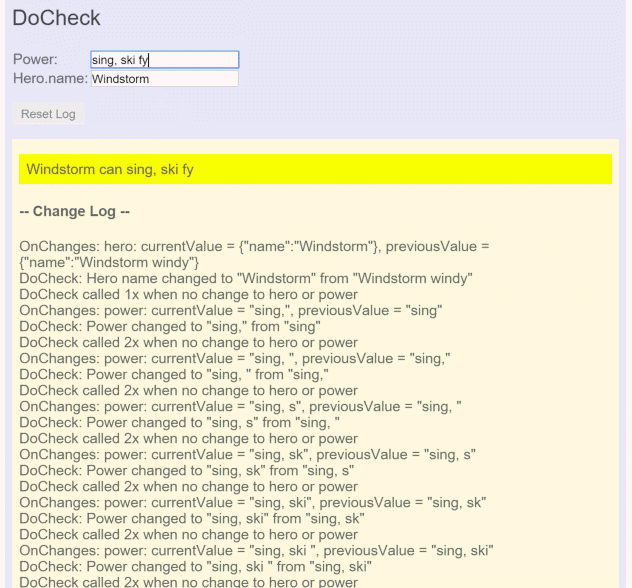
\includegraphics[scale=0.5]{resources/doCheck.png}
 \cite{angular-doc}
    \caption{funzionamento metodo ngDocheck()}
\end{figure}
come si può vedere nell'esempio, il metodo  ngDoCHeck viene chiamato diverse decine di volte anche se non avviene nessuna variazione ai valori dei due campi input.
\newline
Il metodo ngOnInit() è fondamentale nel caso di fetch di dati da un servizio remoto, essendo chiamato alla visualizzazione del componente consente di ritardare il fetch dei dati al momento in cui ce n'è un vero bisogno ed evitare il costoso fetch dei dati da parte del costruttore che rallenterebbe di molto i tempi di load dell'applicazione.
\newline
\newline
Il metodo NgOnDestroy() risulta utile per evitare memory leaks rimuovendo il componente da eventuali emettitori di eventi.

%%%%%%%%%%MODULI
\section{Organizzazione dei componenti, i Moduli}
Uno dei concetti principali del framework Angular è il rendere le applicazioni il più modulari possibile. Per realizzarla la libreria propone il concetto di ngModule, un ngModule consiste in un raggruppamento di entità angular dedicate all'implementazione di una particolare sotto funzionalità, un servizio necessario all'applicazione o un particolare step dell'applicazione.
Un ngModule può contenere al suo interno:
\begin{itemize}
    \item Componenti
    \item Service
    \item Qualunque altro file utile allo sviluppo della funzionalità offerta dal modulo
\end{itemize}
Ogni applicazione Angular è formata da un insieme di ngModule dei quali ne è sempre presente uno radice (root) il quale viene lanciato all'avvio dell'applicazione.
Cosi come i componenti, anche gli ngModule sono organizzati in una struttura ad albero,
della quale la radice è l' ngModule root 
\subsection{Metadati}
un ngModule è definito da una classe typescript con decorator @ngModule il quale definisce i suoi metadati:
\begin{itemize}
    \item La lista di componenti direttive e service che fanno parte del ngModule
    \item Gli elementi che sono visibili e utilizzabili dagli altri moduli
    \item Gli elementi che sono importati da altri moduli
    \item Tutti i fornitori di service che questo modulo espone all'esterno
    \item Il componente root del modulo
\end{itemize}
Ogni ngModule crea un ambiente di compilazione isolato per le entità al suo interno e possiede un componente root che viene caricato al boot, ma è comunque possibile accedere agli altri componenti del ngModule tramite il routing o il rendering del template del singolo componente
\begin{figure}[H]
    \centering
   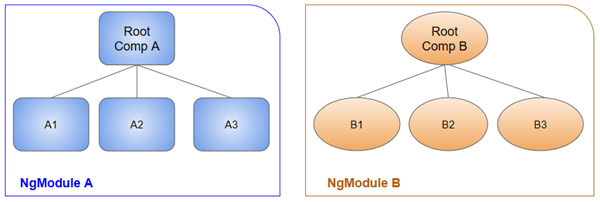
\includegraphics[scale=1]{resources/compilation-context.png}
   \cite{angular-doc}
    \caption{rappresentazione ambiente di compilazione dei moduli}
\end{figure}


come mostrato nell'immagine i due ngModule offrono ambienti di compilazione differenti per i moduli all'interno, questo consente alle applicazioni angular di essere pienamente modulari dato che i singoli moduli sono pienamente indipendenti.
\newline
Come mostrato dall'immagine sottostante, le view possono essere organizzate in gerarchie, che rappresentano singole aree di visualizzazione all'interno della pagina,esse vengono gestite dalla libreria come una unica entità e possono contenere componenti da ngModule differenti
\begin{figure}[H]
    \centering
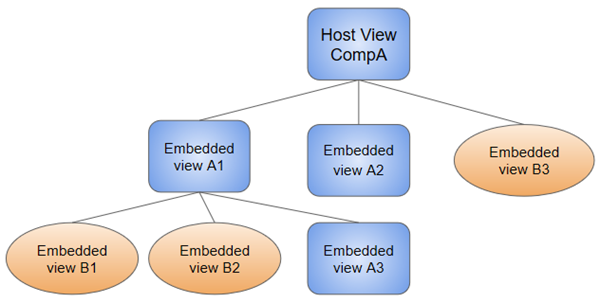
\includegraphics[scale=1]{resources/view-hierarchy.png}
   \cite{angular-doc}
    \caption{rappresentazione gerarchia delle view}
\end{figure}
\newpage

\section{ Implementazione della dependency injection, i Services}
I componenti angular idealmente dovrebbero occuparsi esclusivamente di rendere possibile la user experience costruendo la vista applicativa e sfruttando il data binding per gestire la logica applicativa.
\newline
Per tutti i compiti esterni alla logica applicativa, Angular propone il concetto di Service.
\newline
I Service sono classi typescript descritte dal decorator @Injectable il cui compito è quello di occuparsi delle operazioni di utilità necessarie al funzionamento dei componenti.
Le operazioni gestite dai service possono includere:
\begin{itemize}
    \item Fetch dei dati da datasource esterne
    \item Logging delle operazioni o di debug
    \item Validazione del input utente
\end{itemize}
Grazie ai service è possibile rendere i componenti indipendenti da queste operazioni e rendere riusabile la struttura della vista utente. 
In questo modo i componenti non sono vincolati a particolari sistemi esterni, (ad esempio datasource) che possono avere concezioni di immagazzinamento dei dati differenti.

\subsection{Dependency Injection}
La dependency injection è una funzionalità diventata ormai fondamentale nelle applicazioni enterprise di grandi dimensioni, sia per testing del sistema sia per aumentare la riusabilità e la modularità delle applicazioni. Essa permette di rovesciare la logica di ottenimento delle dipendenze di un particolare componente sofware, liberando il componente dall'obbligo di reperire le dipendenze e delegando a altre entità il compito.
\begin{figure}[H]
    \centering
 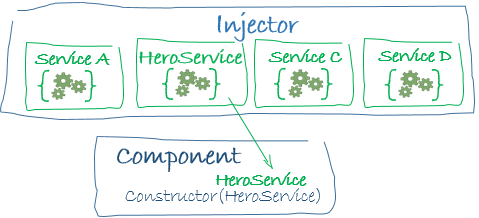
\includegraphics[scale=0.75]{resources/injector-injects.png}
\cite{angular-doc}
   \caption{rappresentazione oggetto Injector}
\end{figure}
La libreria Angular implementa questa funzionalità attraverso i service, essi possono essere richiesti dal costruttore di un componente e vengono forniti dal framework alla creazione dello stesso tramite un oggetto chiamato Injector, in questo modo il componente necessita solo di dichiarare il service di cui ha bisogno e non di definirne la logica di funzionamento o di occuparsi della sua creazione o istanziazione.
\newline
\newline
Un service, per poter essere iniettato all'interno di un componente necessita un provider che consente di definire la visibilità del service. 
Quest'ultima può essere:
\begin{itemize}
    \item A livello di componente, in questo caso per ogni istanza dello specifico componente viene creata un istanza del service
    \item A livello di ngModule, in questo modo viene creata una sola istanza per tutti i componenti che fanno parte di quel service
    \item A livello radice, in questa modalità viene creata una sola istanza del service, che viene resa disponibile a tutti i componenti interni all'applicazione
\end{itemize}
La capacità dei provider di limitare la visibilità dei service è fondamentale anche sotto un punto di vista di ottimizzazione delle prestazioni, in quanto consente di istanziare i service solo in caso si utilizzi il componente applicativo che ne ha un effettivo bisogno.
\newpage

\section{Routing dei componenti Angular}
Una delle funzionalità fondamentali per una single page application è la possibilità di navigare tra le varie viste senza interrogare il server per reperire una nuova pagina.
La libreria Angular consente di navigare tra le viste del' applicazione tramite il package routing, distribuito esternamente rispetto al core.
\newline
\newline
La libreria implementa la funzionalità tramite l'oggetto routing, gestito tramite il pattern singleton e creato all'avvio dell'applicazione, l'oggetto è in grado di tradurre gli url in componenti da renderizzare all'interno della pagina.
Le associazioni tra url e componenti vengono effettuate all'interno della definizione del ngModule, tramite il metodo 
\begin{minted}{javascript}
    RouterModule.forRoot();
\end{minted}
al quale viene fornito, come argomento, un array contenete le coppie url componente.
La renderizzazione dell'output del routing angular avviene all'interno della direttiva
\begin{minted}{html}
    <router-outlet></router-outlet>
\end{minted}
Alla fine di ogni ciclo di navigazione, la libreria costruisce un albero per rappresentare lo stato corrente del router, disponibile a tutti i componenti tramite il service Router. 
\newpage
\section{Gestione runtime dei componenti, il meccanismo change detection}
Per consentire l'aggiornamento runtime  del DOM a seguito delle modifiche delle proprietà dei componenti, Angular sfrutta un meccanismo chiamato change detection.
\newline
 La libreria costruisce un albero composto dai componenti renderizzati e, quando viene lanciato il meccanismo di change detection, essa esegue una visita top down dell'albero in cerca dei componenti le quali proprietà sono state modificate e ne renderizza di nuovo la view. Angular esegue questa operazione solo per le proprietà che vengono utilizzate nel template e per ognuna esegue un controllo con il valore precedente.
\newline
\begin{figure}[H]
\centering
   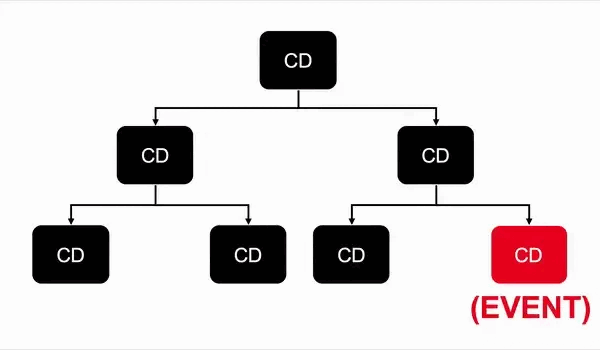
\includegraphics[scale=0.5]{resources/cd-1.png}
\caption{un componente viene modificato e lancia il meccanismo di change detection}
\end{figure}
\begin{figure}[H]
\centering
   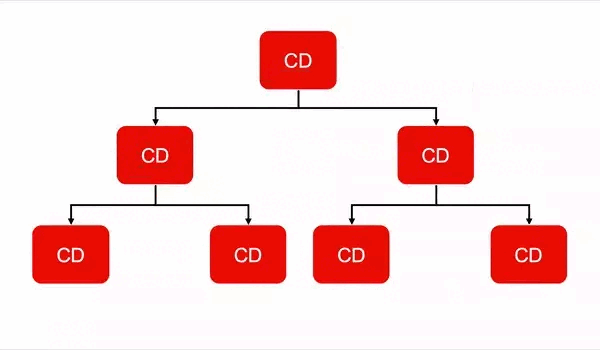
\includegraphics[scale=0.5]{resources/cd-2.png}
\caption{l'albero viene visitato alla ricerca di proprietà modificate}
\end{figure}






\section{Change detection: innesco del meccanismo}

Per poter consentire il corretto avvio del meccanismo la libreria angular modifica il comportamento standard di alcuni metodi di basso livello del motore javascript:
\begin{itemize}
    \item Tutti gli eventi del browser (click, mouseover, keyup, etc. )
    \item Le chiamate ajax HTTP
    \item I metodi setTimeout() e setInterval()
\end{itemize}
Angular inoltre si avvale della libreria zone.js per modificare in maniera trasparente i comportamenti del browser e innescare il meccanismo di change detection come mostrato nell'esempio.
\newline
\begin{minted}{javascript}
        // this is the new version of addEventListener
function addEventListener(eventName, callback) {
     // call the real addEventListener
     callRealAddEventListener(eventName, function() {
        // first call the original callback
        callback(...);     
        // and then run Angular-specific functionality
        var changed = angular.runChangeDetection();
         if (changed) {
             angular.reRenderUIPart();
         }
     });
}

\end{minted}
\cite{angular-doc}


\section{Cange detection: strategie}
Il meccanismo di change detection può avvenire in due principali strategie
\begin{itemize}
    \item Default
    \item OnPush
\end{itemize}
La libreria angular adotta la modalità default, che lancia il meccanismo di change detection ogni volta che viene lanciato un evento di interazione con l'utente, questo può portare a cali di prestazione soprattutto con alberi di componenti molto vasti.
È possibile modificare la strategia di change detection utilizzata all'interno della diretiva Compontent
\begin{minted}{typescript}
    @Component({    selector: 'hero-card',    
    changeDetection: ChangeDetectionStrategy.OnPush,    
    template: ...
    })
    export class HeroCard {    ...}
\end{minted}
I componenti che sfruttano la strategia onPush vengono aggiornati solo nei seguenti casi
\begin{itemize}
    \item Vengono modificati i riferimenti delle proprietà utilizzate nel template
    \item Viene lanciato un evento dal componente o da uno dei suoi figli 
    \item Un oggetto osservabile collegato al template emette un nuovo evento
    \item La change detection viene attivata manualmente
\end{itemize}

\begin{figure}[H]
    \centering
 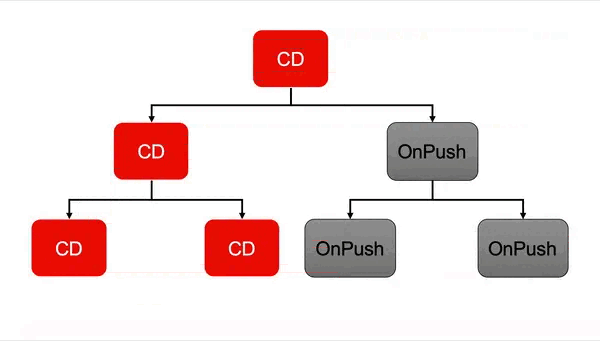
\includegraphics[scale=0.75]{resources/cd-onPush.png}
   \caption{Ciclo di change detection con componenti che sfruttano la strategia onPush}
\end{figure}
In questo modo è possibile evitare che il meccanismo di change detection venga eseguito su componenti di cui non è necessario effettuare sempre l'aggiornamento e rendere l'applicazione più responsiva.
\newline
La strategia onPush tuttavia prevede alcune accortezze per essere utilizzata correttamente. Per come è strutturata la strategia è necessario fornire al template una nuova istanza delle proprietà per poter attivare il meccanismo invece di modificare i valori associati alle proprieta.
\newline
Tuttavia gli oggetti javascript nascono come oggetti mutabili, questo comportamento del linguaggio facilita il manifestarsi di comportamenti non voluti da parte del meccanismo di Change dectection, è consigliabile quindi utilizzare librerie javascript che forniscano oggetti immutabili, come per esempio Immutable.js
%%%%%%% YOU COOK %%%%%%%%%%%%%%%% 
\chapter{Angular: L'applicazione youCook}
\begin{figure}[H]
    \centering
 
\includegraphics[scale=0.2]{resources/youCook_logo.jpg}
   \caption{logo dell'applicazione}
\end{figure}
\newpage
\section{YouCook: requisiti}
Al fine di mostrare le potenzialità della libreria segue il progetto di una applicazione per la gestione e condivisione delle ricette di cucina.
L' applicazione vuole soppiantare il classico "Libro mastro delle ricette" offrendo la possibilità di monitorare, aggiornare e gestire il proprio repertorio di ricette.
I requisiti della applicazione sono i seguenti:
\begin{itemize}
    \item L'utente deve poter gestire le proprie ricette, modificarle, creare e eliminarti
    \item L'utente deve poter effetuare ricerche in base agli ingredienti principali delle ricette
    \item L' utente deve poter creare gruppi famiglia all'interno dei quali selezionare fra le ricette il "Pasto del giorno" ovvero la ricetta che si intende realizzare per il pasto selezionato "pranzo, cena"
    \item all'interno del gruppo famiglia l'utente deve poter amministrare i membri 
    
\end{itemize}
L'applicazione ha inoltre come obbiettivo quello di mettere in luce le potenzialità della strategia di change detection onPush.
\newpage
\subsection{Tabella dei requisiti}
\FloatBarrier
\begin{longtable}{|p{2.5cm}|p{9cm}|p{2.5cm}|}
\hline

\endfirsthead
\multicolumn{3}{c}%
{\tablename\ \thetable\ -- \textit{Continued from previous page}} \\
\hline
 \rowcolor{white}\textbf{ID} & \textbf{REQUISITO} & \textbf{TIPO} \\
\hline
\endhead
\hline \multicolumn{3}{r}{\textit{Continued on next page}} \\
\endfoot
\hline
\endlastfoot

\rowcolor{white}\textbf{ID} & \textbf{REQUISITO} & \textbf{TIPO} \\
         \hline
         R1F &L'applicazione deve fornire una funzionalità di registrazione agli utenti & Funzionale\\
         
         \hline
         R2F &L'applicazione deve dare la possibilità di aggiungere modificare e eliminare le proprie ricette&Funzionale \\
         
         \hline
         R3F &L'acquirente deve poter effettuare ricerche in base agli ingredienti & Funzionale \\
         
         \hline
         R4F &L'applicazione deve poter permettere all'utente di creare gruppi famiglia&Funzionale \\
         
         \hline
         R5F &L'applicazione deve poter permettere all'utente di amministrare i gruppi famiglia, rimuovendo o aggiungendo mebri al gruppo &Funzionale \\
         
         \hline
         R6F & L'applicazione deve consentire all'utente di selezionare il "pasto del giorno"&Funzionale \\

\end{longtable}
\FloatBarrier
\newpage
\begin{figure}[H]
    \centering
 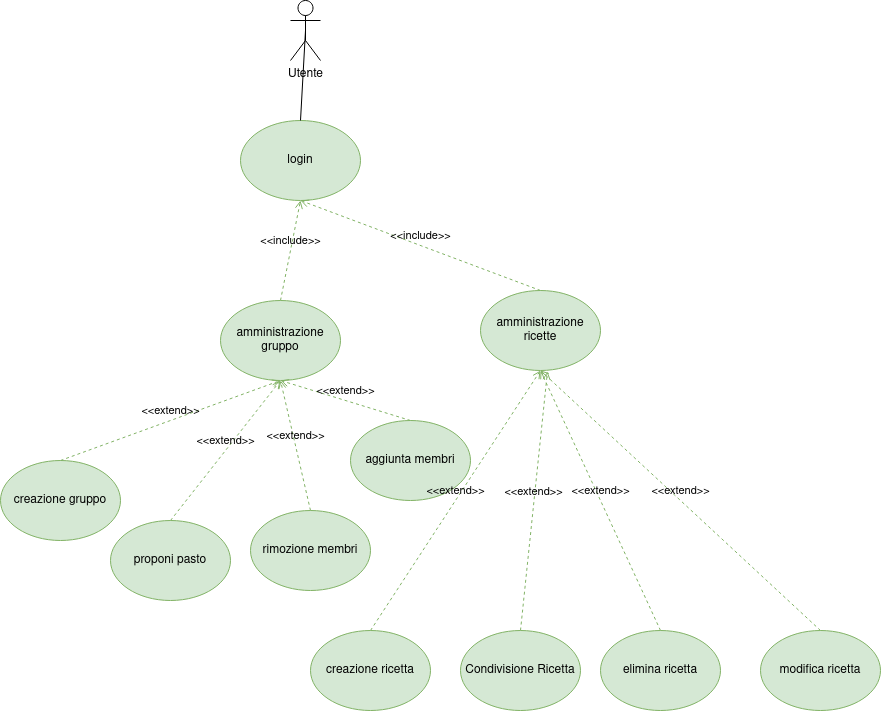
\includegraphics[scale=0.5]{resources/diagramma_casi_uso.drawio.png}
   \caption{Diagramma casi d'uso della applicazione}
\end{figure}
Il diagramma mette in luce le principali funzionalità fornite all'utente che, dopo la procedura di login, può visualizzare il proprio elenco di ricette e interagire con lo stesso  oppure visionare i membri del gruppo famiglia a lui associato.
\section{YouCook: Scenari}

\FloatBarrier
\begin{longtable}{|p{4.5cm}|p{10cm}|}
\hline
\endfirsthead
\multicolumn{2}{c}%
{\tablename\ \thetable\ -- \textit{Continued from previous page}} \\
\hline
\endhead
\hline \multicolumn{2}{r}{\textit{Continued on next page}} \\
\endfoot
\hline
\endlastfoot


         \textbf{Titolo} & Login \\

         \hline
         \textbf{Descrizione} & Permette di accedere al sistema \\

         \hline
         \textbf{Attori} & Utente\\

         \hline
         \textbf{Relazioni} & Amministrazione gruppo, Amministrazione ricette \\
         \hline
         \textbf{Precondizioni} & L'utente deve essere già registrato\\

         \hline
         \textbf{Postcondizioni} & L'utente è autenticato nel sistema\\

         \hline
         \textbf{Scenario principale} & 
            \begin{enumerate}
                \item All'utente viene presentata una maschera per l'inserimento delle credenziali
                \item L'utente inserisce i propri dati
                \item Il sistema verifica che i dati inseriti siano corretti
                \item Viene presentata la schermata principale all'utente 
            \end{enumerate}
            \\


         \hline
         \textbf{Scenari alternativi} & Scenario a: Credenziali non riconosciute
            \begin{enumerate}
                \setcounter{enumi}{3}
                \item Il sistema non riconosce le credenziali inserite e presenta nuovamente la schermata iniziale di accesso
            \end{enumerate}
         \\

         \hline
         \textbf{Requisiti non funzionali} &\\

         \hline
         \textbf{Punti aperti} & \\



\end{longtable}
\FloatBarrier
\begin{longtable}{|p{4.5cm}|p{10cm}|}
\hline
\endfirsthead
\multicolumn{2}{c}%
{\tablename\ \thetable\ -- \textit{Continued from previous page}} \\
\hline
\endhead
\hline \multicolumn{2}{r}{\textit{Continued on next page}} \\
\endfoot
\hline
\endlastfoot


         \textbf{Titolo} & Amministrazione ricette \\

         \hline
         \textbf{Descrizione} & Permette di eliminare, modificare e aggiungere ricette  \\

         \hline
         \textbf{Attori} & Utente\\

         \hline
         \textbf{Relazioni} & creazione ricetta, modifica ricetta, elimina ricetta, login \\
         \hline
         \textbf{Precondizioni} & L'utente deve essere già autenticato\\

         \hline
         \textbf{Postcondizioni} &L'utente ha modificato il suo elenco di ricette\\

         \hline
         \textbf{Scenario principale} & 
            \begin{enumerate}
                \item All'utente viene presentata una maschera con all'interno la lista delle ricette presenti nel suo inventario 
                \item L'utente seleziona l'opzione che vuole effettuare (modifica, aggiunta o eliminazione)
                \item Il sistema porta a compimento l'azione descritta dall'utente
            \end{enumerate}
            \\


         \hline
         
         \hline
         \textbf{Requisiti non funzionali} &\\

         \hline
         \textbf{Punti aperti} & \\



\end{longtable}
\FloatBarrier
\begin{longtable}{|p{4.5cm}|p{10cm}|}
\hline
\endfirsthead
\multicolumn{2}{c}%
{\tablename\ \thetable\ -- \textit{Continued from previous page}} \\
\hline
\endhead
\hline \multicolumn{2}{r}{\textit{Continued on next page}} \\
\endfoot
\hline
\endlastfoot


         \textbf{Titolo} & Amministrazione Gruppo famiglia \\

         \hline
         \textbf{Descrizione} & Permette di eliminare e aggiungere mebri al gruppo famiglia  \\

         \hline
         \textbf{Attori} & Utente\\

         \hline
         \textbf{Relazioni} & aggiunta membro, rimozione membro, login \\
         \hline
         \textbf{Precondizioni} & L'utente deve essere già autenticato\\

         \hline
         \textbf{Postcondizioni} &L'utente ha modificato il suo gruppo famiglia\\

         \hline
         \textbf{Scenario principale} & 
            \begin{enumerate}
                \item All'utente viene presentata una maschera con all'interno la lista dei mebri del suo gruppo famiglia 
                \item L'utente seleziona l'opzione che vuole effettuare (aggiunta o eliminazione)
                \item Il sistema porta a compimento l'azione descritta dall'utente
            \end{enumerate}
            \\


         \hline
         
         \hline
         \textbf{Requisiti non funzionali} &\\

         \hline
         \textbf{Punti aperti} & \\



\end{longtable}
\section{YouCook: modello del dominio}
\begin{figure}[H]
    \centering
 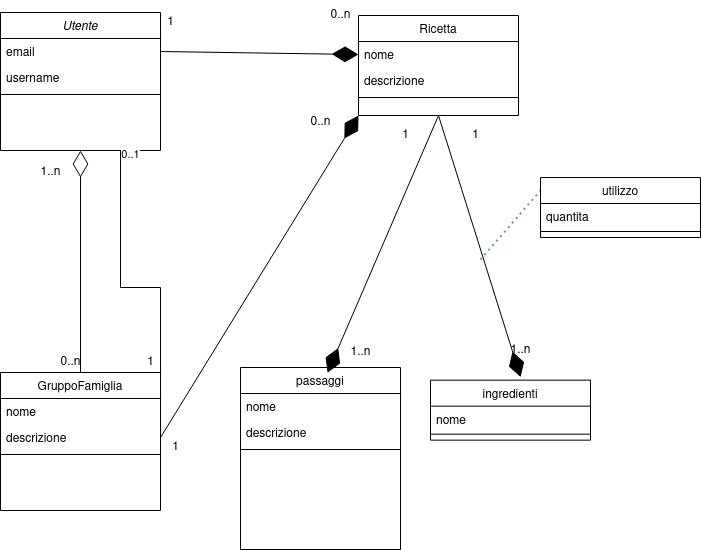
\includegraphics[scale=0.7]{resources/modello_del_dominio.drawio.png}
   \caption{Modello del dominio dell'applicazione}
\end{figure}
Il modello del dominio sopra rappresentato definisce le entità in gioco nell'applicazione. In particolare, vengono sfruttate due realazioni tra le classi utenti e gruppo famiglia per rappresentare i membri e il proprietario del gruppo. Viene inoltre utilizzata una classe d'associazione per rappresentare l'utilizzo del dato ingrediente in quella ricetta.
\section{YouCook: progettazione}
La struttura dell'applicazione è la seguente
\begin{figure}[H]
    \centering
 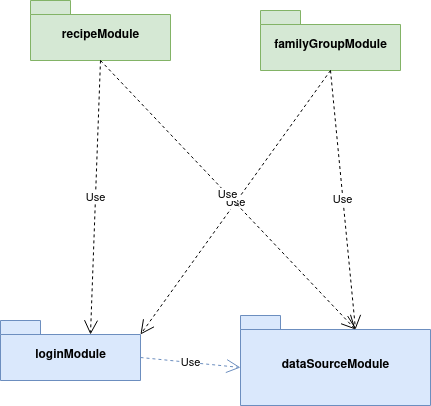
\includegraphics[scale=0.7]{resources/diagramma_package-diagramma_package.drawio.png}
   \caption{Diagramma dei package dell'applicazione}
\end{figure}
L'applicazione è composta da 4 module: i module recipe e familygroup implementano le rispettive funzionalità e sfruttano i servizi offerti dai module login e dataSource per autenticare gli utenti e realizzare la persistenza dei dati. 
\begin{figure}[H]
    \centering
 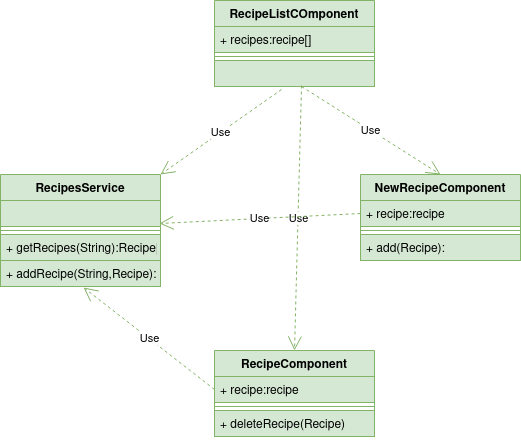
\includegraphics[scale=0.7]{resources/diagramma_package-recipe.drawio.png}
   \caption{Diagramma delle classi pakage recipe}
\end{figure}
 
\begin{figure}[H]
    \centering
 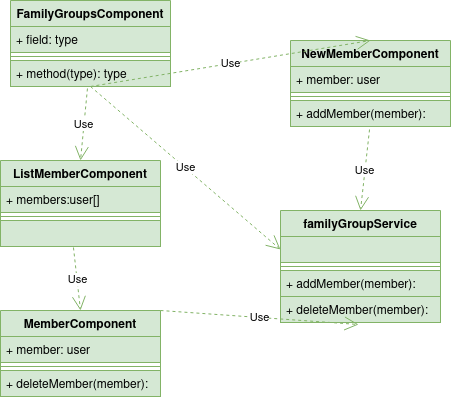
\includegraphics[scale=0.7]{resources/diagramma_package-FamilyGroup.drawio.png}
   \caption{Diagramma delle classi pakage FamilyGroup}
\end{figure}
I componenti dei package Recipe e FamilyGroup sfruttano la strategia di change detection onPush per aggiornare la lista di elementi mostrate nella view e sfruttano i rispettivi Service per interagire con la lista di elementi. Questi ultimi restituiscono a ogni modifica una nuova istanza della lista per attivare il meccanismo  di change detection.
\newline
È stato deciso di delegare la gestione della generazione degli oggetti a un service apposito, cosi da sollevare i componenti dalla necessità di implementare la logica applicativa. In questo modo i componenti possono concentrarsi sulla gestione della interfaccia e in caso si necessiti di modificare la logica con cui vengono gestiti i dati sarà sufficiente agire sul service.
\newpage
\begin{figure}[H]
    \centering
 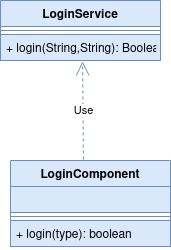
\includegraphics[scale=0.7]{resources/diagramma_package-login.drawio.png}
   \caption{Diagramma delle classi pakage login}
\end{figure}
\begin{figure}[H]
    \centering
 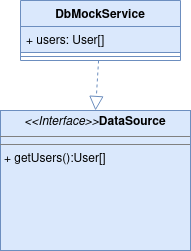
\includegraphics[scale=0.7]{resources/diagramma_package-dataSource.drawio.png}
   \caption{Diagramma delle classi pakage dataSource}
\end{figure}
Il package DataSource sfrutta il pattern strategy per implementare la persistenza verso i data store tramite l'interfaccia DataSource. In questo modo si astrae l'applicazione dalla gestione dello storage dei dati e consentire il recupero dei dati da datastore differenti.
\newline
I package login e datasource mettono ha disposizione una classe service per fornire le funzionalità agli altri componenti.




%- capitolo 1 e capitolo 2 vanno abbastanza bene, mentre il capitolo 3 è deboluccio.
%Riporti anche motivazioni più estese delle scelte fatte, screenshot dell'applicazione realizzata che la aiutino a descriverne le funzionalità. Servirebbero anche dati numerici sulle prestazioni di performance, ma forse a questo punto non ha più il tempo di farle...
\section{YouCook: interfacce}
di seguito si riporta l'interfaccia principale della applicazione

\begin{figure}[H]
    \centering
 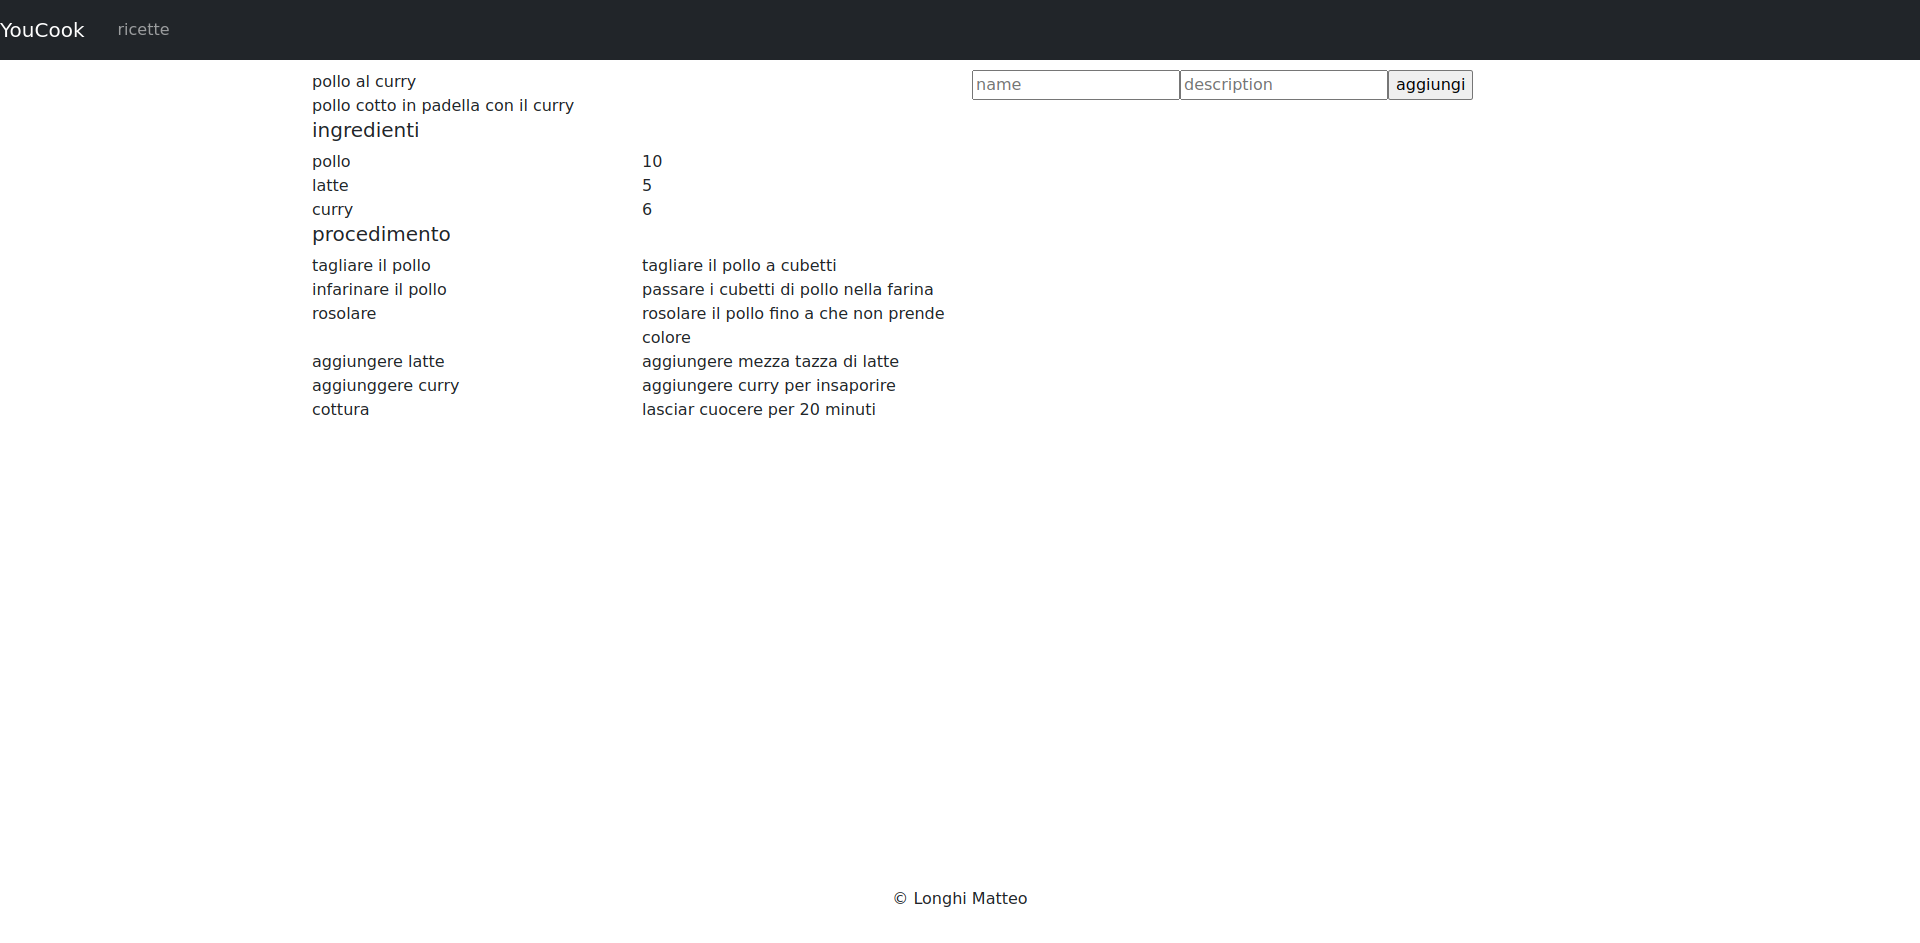
\includegraphics[scale=0.2]{resources/interfaccia-recipes.png}
   \caption{interfaccia sezione recipes dell'applicazione}
\end{figure}
L'interfaccia offre la possibilità di visionare l'elenco delle ricette e di aggiungerne di nuove tramite il form apposito.
L'elenco a destra viene renderizzato tramite la strategia onpush di change detection.
\newline
Il componente RecipesListComponent si registra a un osservabile messo a disposizione dal RecipesService che, alla modifica della lista di ricette da parte del NewRecipeComponent, emette una nuova lista di ricette attivando cosi il meccanismo di change detection
\newpage
codice NewRecipeComponent:
\begin{minted}{typescript}
import { ChangeDetectionStrategy, Component, OnInit } from '@angular/core';
import { Recipe } from '../model/Recipe';
import { RecipesService } from '../recipes.service';

@Component({
  selector: 'app-recipes-list',
  changeDetection:ChangeDetectionStrategy.OnPush,
  templateUrl: './recipes-list.component.html',
  styleUrls: ['./recipes-list.component.css']
})
export class RecipesListComponent implements OnInit {
  public recipes?:Recipe[];
  constructor(private rs:RecipesService ){
  }
  ngOnInit(): void {
   this.recipes=this.rs.getRecipes();
   this.rs.recipesEvent.subscribe(recipes=>{
    this.recipes=recipes
   })
  }
  

}

\end{minted}

\newpage
codice RecipeService;
\begin{minted}{typescript}
import { EventEmitter, Injectable } from '@angular/core';
import { DatabaseService } from 'src/database.service';
import { Recipe } from './model/Recipe';
import { SessionService } from './session.service';

@Injectable({
  providedIn: 'root'
})
export class RecipesService {
private recipes?:Recipe[];
public recipesEvent:EventEmitter<Recipe[]>=new EventEmitter();
  constructor(private dbs:DatabaseService, private ss:SessionService ) { 
    this.recipes=this.dbs.getUser(this.ss.getUsername())?.recipies;
  }
  public getRecipes(){
    return JSON.parse(JSON.stringify(this.recipes));

  }
  public addRecipes(r:Recipe ){
    this.recipes?.push(r);
   
    this.recipesEvent.emit(this.recipes);
    
  }
}
\end{minted}

\section{YouCook: test prestazioni}
Sono stati anche eseguiti dei test sull'applicazione per verificarne i tempi di risposta
\begin{figure}[H]
    \centering
 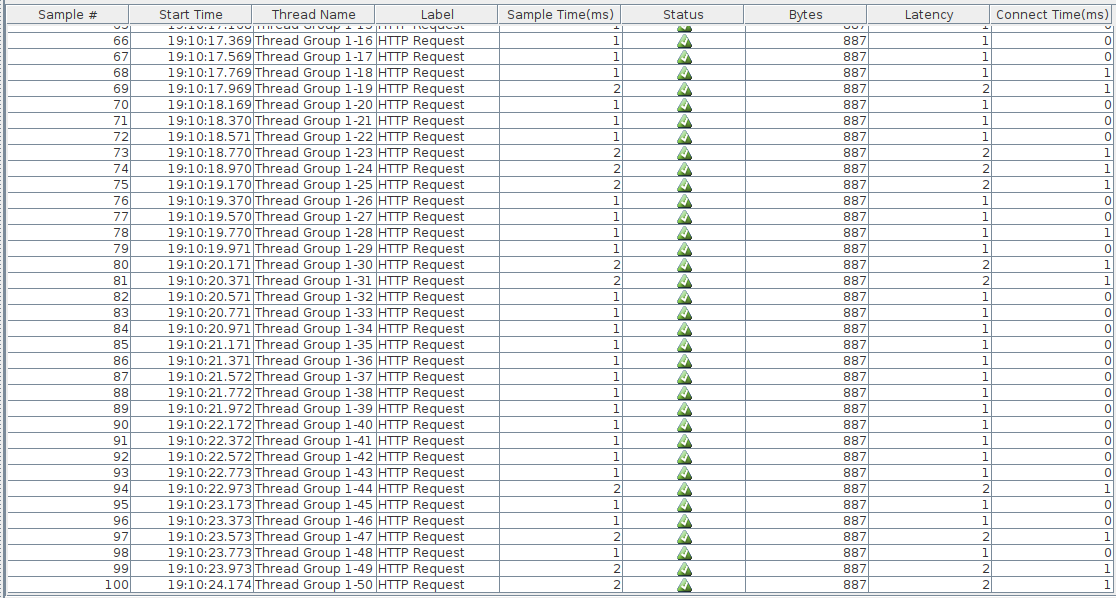
\includegraphics[scale=0.4]{resources/tests.png}
   \caption{Test effettuati per mezzo di jmeter}
\end{figure}
Il test eseguito prevedeva un pool di 50 thread, dal quale possiamo evincere che l'applicazione si comporta egregiamente sotto carico, totalizzando un tempo medio di risposta di circa 2 millisecondi (l'applicazione è stata testata in una rete locale)




%%%%%%%%%% Conclusions %%%%%%%%%%
\newpage
\thispagestyle{empty}
\mbox{}
\newpage

\addcontentsline{toc}{chapter}{Conclusioni}
\chapter*{Conclusioni}

Come mostrato nell'elaborato, le prestazioni in termini di tempo di risposta delle applicazioni sono cruciali quando si vuole fornire una valida user experience. L'utente moderno del web vuole applicazioni responsive e non desidera perdere tempo dietro a schermate di caricamento. In un contesto simile l'ottimizzazione delle prestazioni deve essere un punto cruciale dello sviluppo delle applicazioni web sin dalle prime fasi del progetto.
\newline
In questo contesto la libreria Angular si è evoluta molto dalla sua prima creazione nel 2016. Essa offre una suite di concetti completa e all'avanguardia, in grado di soddisfare le necessità di sviluppo di applicazioni complesse e data intensive senza sacrificare le prestazioni.
\newline
Il concetto di componente proposto dalla libreria suddivide la visualizzazione dei dati e la logica applicativa dalla rappresentazione a schermo in maniera ottimale, consente di fare dialogare i due mondi agilmente tramite il data binding, sollevando lo sviluppatore da questo compito e consente di limitare la progettazione del componente solo a questi due aspetti, delegando altri compiti di utilità a concetti diversi come i service.
\newline 
La libreria non si risparmia nell'implementazione del concetto di modularità e tramite i module è possibile realizzare applicazioni composte da elementi assestanti e in grado di essere importati in altre applicazioni e utilizzati in maniera autonoma.
\newline
La dependency injection fornita dall'applicazione tramite il concetto di service rende i componenti ignari delle logiche di utilità necessarie all'applicazione per funzionare, questo consente di pensare i componenti come compartimenti stagni che, tramite i service, si interfacciano con il resto dell'applicazione.
\newline 
La capacita di influenzare il ciclo di vita dei componenti e il meccanismo di change detection consentono di effettuare un preciso tuning delle prestazioni e della gestione degli eventi a runtime dell'applicazione, questo offre allo sviluppatore un ambiente runtime molto performante e con una alta possibilità di personalizzazione per adattarsi alle esigenze della applicazione. Il meccanismo di change detection può essere letteralmente modellato "addosso all'applicazione" definendo, per ogni componente, come l'ambiente a runtime deve comportarsi per eseguire l'aggiornamento dell'interfaccia.
\newline 
La libreria, nell'ottica di ridurre al minimo il tempo speso per operazioni di corredo, offre inoltre un vasto ambiente per la generazione del codice e per il testing delle applicazioni.
\newline 
L'applicazione YouCook mostrata nell'elaborato e sviluppata sfruttando le funzionalità offerte dal framework, consente di amministrare la propria libreria di ricette fornendo una versione elettronica del tradizionale ricettario di carta.
Grazie ai concetti offerti dal framework la progettazione risulta facilmente estendibile e modulare consentendo di variare il datastore e di estendere le interfacce tramite l'aggiunta di componenti e service.
\newline 
Per queste motivazioni la libreria Angular si dimostra una delle migliori soluzioni per lo sviluppo di applicazioni web ad alte prestazioni.



%%%%%%%%%% Bibliography %%%%%%%%%%%
\newpage

\printbibliography



\end{document}